%%
%%  chapter02.tex - Obstacle Detection and Planning for Autonomous Vehicles based on Computer Vision Techniques
%%
%%  Copyright 2014 Néstor Morales <nestor@isaatc.ull.es>
%%
%%  This work is licensed under a Creative Commons Attribution 4.0 International License.
%%

\graphicspath{{./images/chapter02/bmps/}{./images/chapter02/vects/}{./images/chapter02/}}

\chapter{Change detection for obstacle localization in images}\label{ch:chapter02}

We drive by mind. That is, once we learn the path to go from a point $A$ to another point $B$, we follow that path without almost thinking. Even more, if a person does this way repeatedly and every day, there will be a day in which he will be able to memorize each black spot, each traffic light and even each pothole. So it is not difficult for us to be surprised the day in which they change the signals or the sense of a road.
Following this line of thought, we have developed a system in which we make our prototype to \emph{learn} the environment of a certain road, making it able to detect the changes. However, in our case, the changes in which we are interested are the obstacles in the way of the vehicle, giving it the ability to avoid them or to stop if necessary. The idea behind this system is having a dataset with images that have localization information associated. These images will be compared with those captured in real time by the on board cameras. Both images will be registered and changes detected, letting us to know the presence of obstacles or other changes that appeared since the stored images were captured.

This is done through the pipeline shown at figure \ref{fig:cp02_pipeline}. First, the database is captured offline. Then, in real time, images are aligned trough a typical image registration pipeline(feature localization, matching of the features between the images, image transformation and resampling). With the images aligned,  obstacles are retrieved.

\begin{figure}[thb]
  \centering
  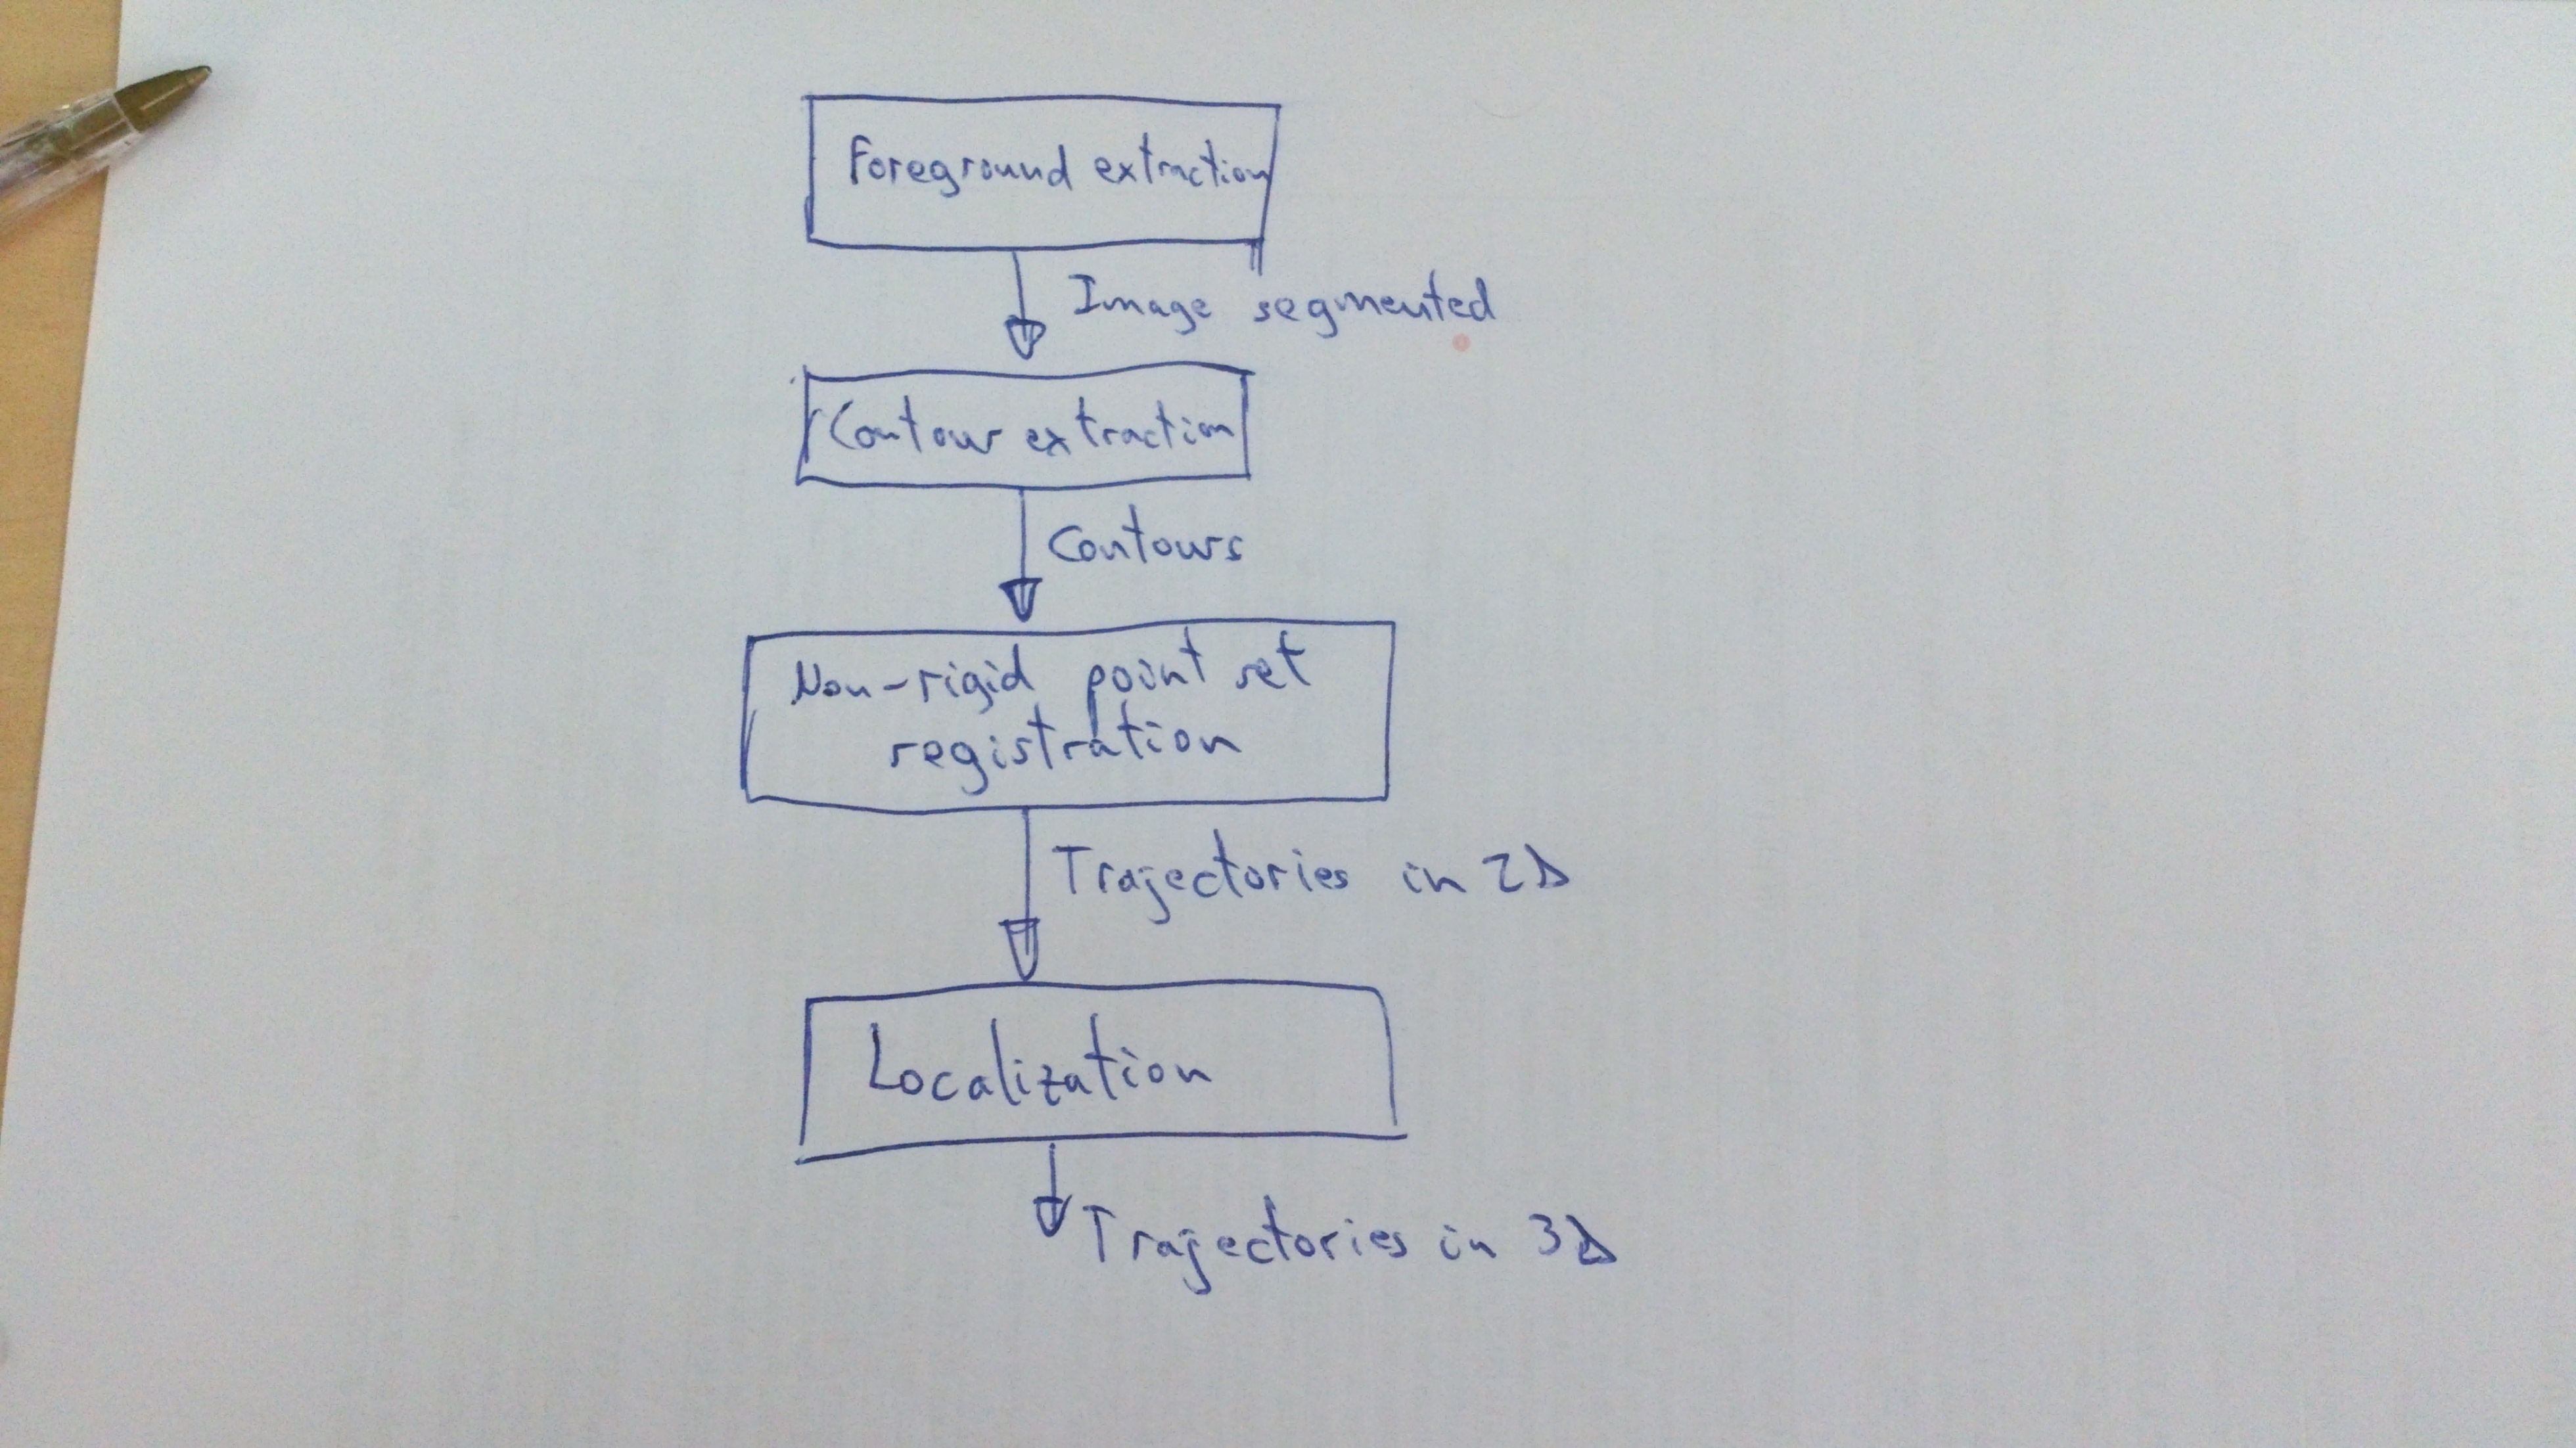
\includegraphics{pipeline}
  \caption{Pipeline of the method.}
  \label{fig:cp02_pipeline}
\end{figure}

\section{The Method}\label{ch:chapter02_01}

In this section, we will describe each of the stages in the pipeline of the application, starting from the database generation and finishing with the detected obstacles. 

As said, the process is based on the generation of an image database in which each image is associated with certain meta-information, of which a big part is related to its position in the map, so the first step in the application is the development of a database covering the driving area. In this stage, the vehicle will be traveling inside the covered area, driven by a human or in controlled circumstances. While the vehicle is driven, the system stores images, which will have associated geographic information: \emph{latitude}, \emph{longitude}, \emph{height} and their transformation into $x$, $y$, $z$ and orientation coordinates with respect to the coordinates frame of the local map of the prototype. Other information that could be outstanding in the future is also stored (i.e., the day and the hour in which the image was taken, GPS rms value, etc.). Images are pre-processed to have as information as possible when used in the next phase, reducing the execution times. For example, we get the set of features from the images offline, not in the real time application. With a $5\,Hz$ update rate, an image is stored about each meter traveled, depending on the speed of the vehicle. In this phase, there would not be any obstacle in the road where the car is going to drive. If so, in the later phase in which the images are processed to get the obstacles, fake objects are going to be detected, due to those obstacles recorded in the database image. Once this process is finished, there will be a database with geographically located images. In figure \ref{fig:cp02_image_database}, a composition of the testing area with some of the stored images highlighted is shown.

\begin{figure}[thb]
  \centering
  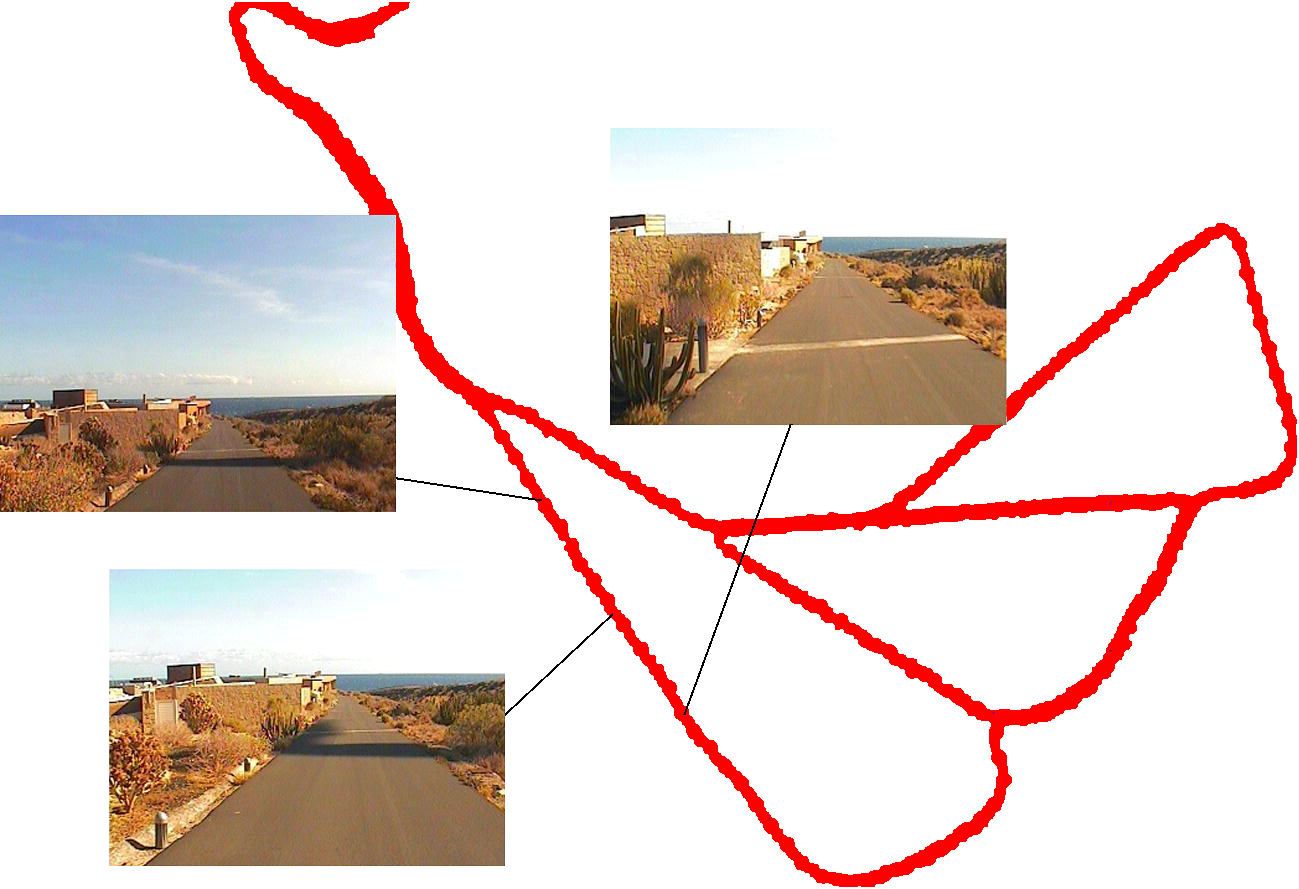
\includegraphics{database}
  \caption{Area covered by the database with some example images superimposed.}
  \label{fig:cp02_image_database}
\end{figure}

In real time, the vehicle starts driving by itself. Along the path, it passes over different positions near the recorded route. These positions are being reported by the GPS device and transformed to the local coordinates to work easily with them. Simultaneously, an image is obtained from the camera while the system looks for the nearest image in the database. The current frame $I_{RT}$ and the image retrieved from the database $I_{DB}$ are compared by using image change detection techniques, obtaining the obstacles in the scene.

In the moment of the development of this application, localization was entirely retrieved from the GPS device. This gave a position each 200 ms, so it was desirable to be able to process each frame under this time, in an on board 2009 PC computer.

\subsection{Image selection from database}\label{ch:chapter02_01_01}

This step is important as we want to get an image as similar as possible to the current real time image. This will affect to the quality of the adjustment between the images. Most of the times we just need to find an image with the smaller Euclidean distance to the current point, checking that the angular difference is not too big. Although this solution has good results, many times it is better to have an image not so close to the current point, if it means that all the objects represented in an image are going to appear in the other one. This can be got if an image which is forward or backward regarding to the current image is selected, so one of the images will be contained into the other. Doing that, it will reduce not just the angular difference, but also the lateral distance (which is usually the source of the misalignments due to an excess of parallax).

In figure \ref{fig:cp02_nearest_image}, we can observe this procedure. Based on this, the nearest image in the database is that obtained by the expression:

\begin{equation}\label{eq:cp02_nearest_image}
I^*_{DB} = \underset{I_{DB}}{\arg\min} \|p_{RT} - p_c\| = {{y_{RT} \cdot v_{DB_x} + x_{RT} \cdot v_{DB_y}} \over 
  {v_{DB_y} \cdot cos(\theta_{RT}) - v_{DB_x} \cdot sin(\theta_{RT})}}
\end{equation}

There, $p_{RT} = (x_{RT}, y_{RT})$ is the position of the vehicle, $p_{DB_i} = (x_{DB_i}, y_{DB_i})$ is the position of each of the images in the database, and $p_c = (x_c, y_c)$ is the crossing point shown at figure \ref{fig:cp02_nearest_image}; $v_{DB_x} = x_{DB} + cos(\theta_{DB})$ and $v_{DB_y} = y_{DB} + sin(\theta_{DB})$; and 
$\theta_{RT}$ and $\theta_{DB_i}$ are the orientations of the vehicle and each of the images in the database. At the end of this selection process a pair of images will be obtained: the current frame, and the associated image extracted from the database. At the same time, we get other related information from the database, like masks, control points, and other things previously computed.

\begin{figure}[thb]
  \centering
  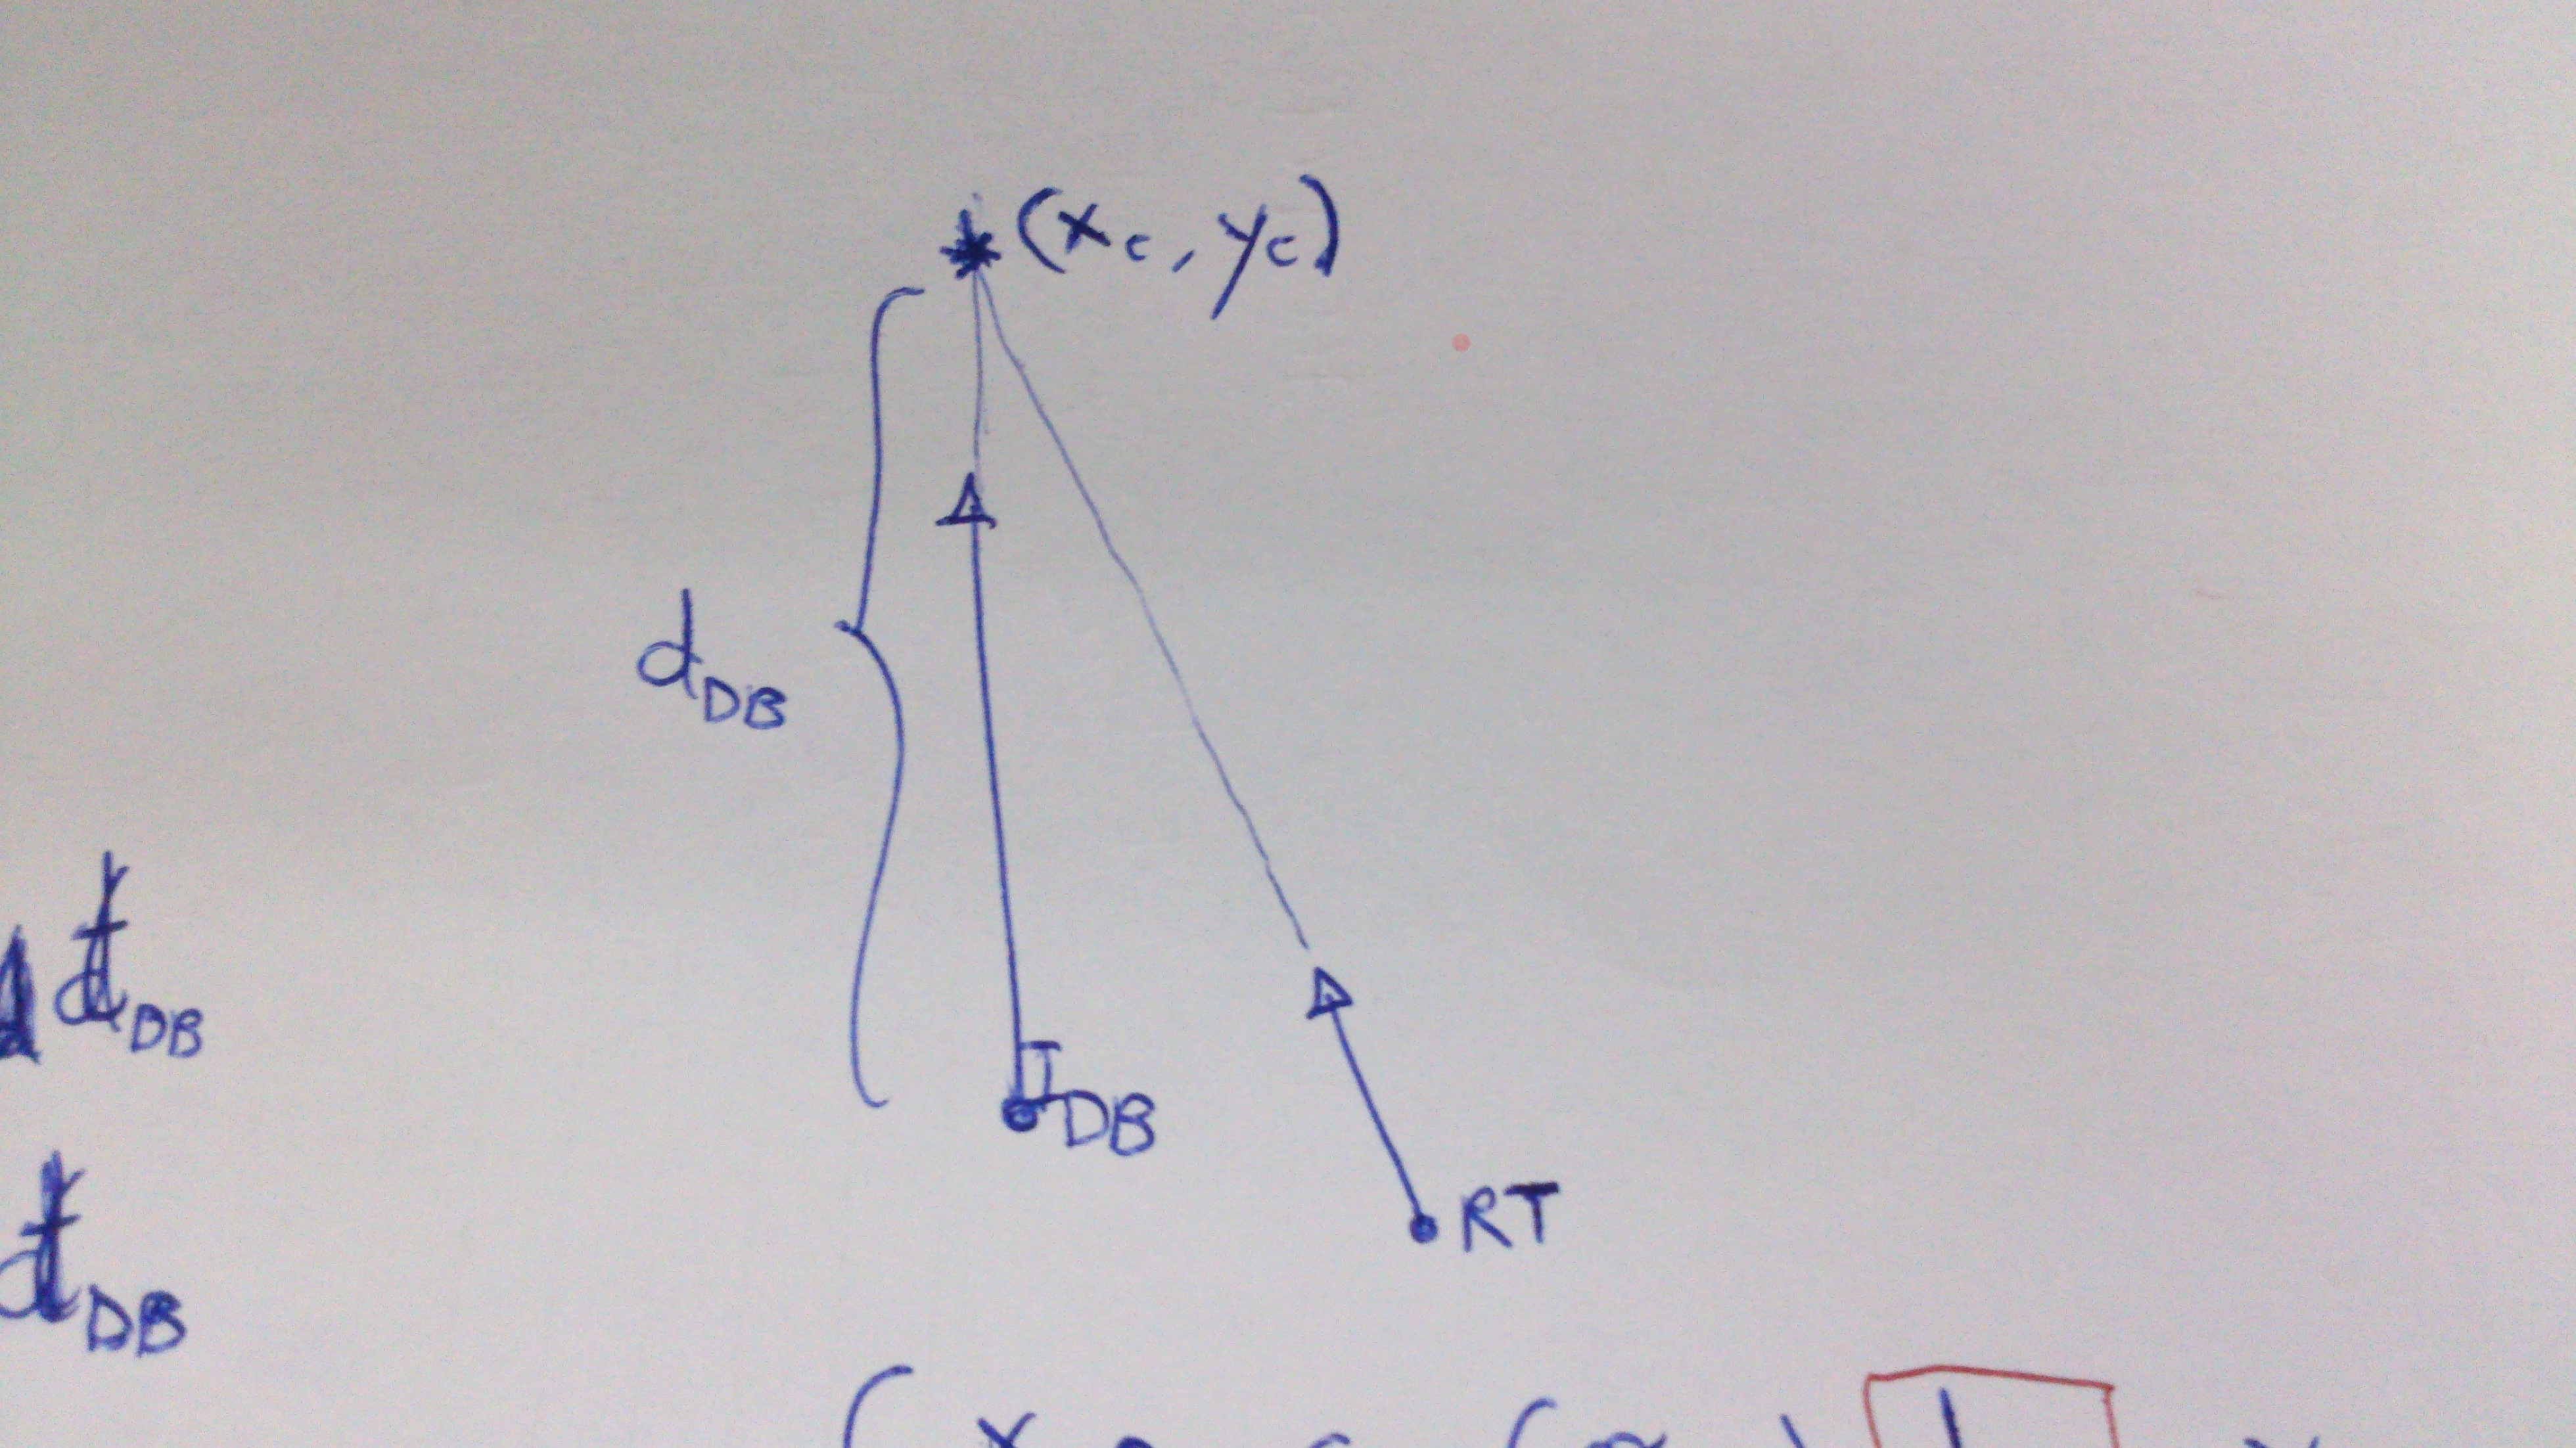
\includegraphics{nearest_image}
  \caption{Nearest image is retrieved.}
  \label{fig:cp02_nearest_image}
\end{figure}

With the aforementioned method for image selection, it is ensured that the image content is going to be similar in both images based on their geographical associated points. However, as it will be seen in the next sections, the methods employed for the adjustment and comparison of these images are sensitive to illumination changes or other problems caused by shadows or different atmospheric conditions. For this purpose, some extra values are included into the database. These values are the date and the hour in which the image was taken.

Using this information, it is possible to limit the number of images to those in which the external conditions are going to be similar to the current. That is, during the day, the sun is moving and causing different shadows and lights at different times of the day. Different shadows can be considered as fake obstacles by the algorithm, so it would be desirable to compare just images in which shadows are not very different. Also changes in the brightness of the images could affect to the detection and matching of similar features in both images. To avoid this, just the images in the set $A$ are eligible:

\begin{equation}\label{eq:cp02_eligible_images_by_time}
A = \{ \forall I_{DB} ~|~ diff\_ToD(I_{DB}, I_{RT}) < \tau_{ToD} \wedge diff\_DoY(I_{DB}, I_{RT}) < \tau_{DoY} \}
\end{equation}

, where $I_{DB}$ is each of the retrievable images from the database; $diff\_ToD(I_1, I_2)$ is a function that retrieves the difference in seconds of the \emph{Time of the Day} in which images $i_1$ and $I_2$ were captured; $diff\_DoY(I_1, I_2)$ is a function that retrieves the difference in days of the \emph{Day of the Year} in which images $i_1$ and $I_2$ were captured (with this, we ensure that we are using images taken in similar seasons of the year, with similar lighting conditions). $\tau_{ToD}$ and $\tau_{DoY}$ are free parameters that limit the size of the set $A$.

However, despite of the fact that for most of the cases selecting reference images inside the $A$ set is enough to ensure a good behavior of the method, we can be more restrictive. Even with the selection presented in $A$, illumination can be different in many cases. To minimize this, there is another parameter, the brightness, which is stored in the database for a fast retrieval. With this parameter, just images inside the following set will be retrieved:

\begin{equation}\label{eq:cp02_eligible_images_by_brightness}
B = \{ \forall I_{DB} ~|~ \| \mu_{RT} - \mu_{DB} \| < \tau_{\mu} \}
\end{equation}

, where $\mu_{RT}$ and $\mu_{DB}$ are the brightness values for the current image and an image in the database, and $\tau_{\mu}$ is a user defined parameter that limits the size of set $B$. Experimentally, best results are obtained when $\tau_{\mu}$ is below 20\%. An study of the influence of this threshold is presented at section \ref{ch:chapter02_02_01}. Finally, from $A$ and $B$ we obtain the group

\begin{equation}\label{eq:cp02_eligible_images}
C = A \cap B
\end{equation}

, which will be the input set of images in the retrieval process. $\tau_{DoY}$ and $\tau_{\mu}$ are interrelated. That is, it is needed to have enough images in the set $A$ in order to be sure that $C \neq \emptyset$ when after intersecting it with $B$. To ensure that, images from different days should be chosen in order to ensure that we find an image with similar illumination conditions to the current frame in the surroundings of the vehicle.

\subsection{Image registration}\label{ch:chapter02_01_02}

In this step, a pair of images which represents the same scene, but taken from different view points, moments and cameras, will be superimposed.

This kind of techniques are well known and very used for a big quantity of tasks, like multi-spectral classification, change detection, image stitching, etc., as reflected at \cite{kooper2011stitching, singh1996digital, coppin1996digital, radke2005image, zitova2003image}.

In general, registration techniques have problems with image disparities due to the movement of non static objects (windmills, flags, etc.). Other problems are caused by the shadows or the reflections that are different depending on the position of the source of the light (for example, the position of the sun during the day for images taken out of a building), or the point of view from where the images where taken, as well as changes in the objects in the course of the time (like the fruit that get rotten or a bush flowering). All these changes can produce problems depending on the features that are expected to be detected.

Most of the registration methods use the following steps: feature detection, feature matching, transformation model estimation, and image resampling and transformation. Same steps have been used in our method.

\subsubsection{Feature detection}\label{ch:chapter02_01_02_01}

The first step consists on the detection of similar features in both images to be able to match them in a later step. Therefore, it is needed that, for the same scene, the detected features in one image and the other to be the same, regardless of the effect of perspective, rotation, hidden objects and brightness and contrast changes. One of the first things that must be decided is which kind of features are going to be used, being the most used the features based on corners, borders and areas (\cite{li2008comprehensive}). To develop this method, some tests have been made with corners and area based methods. After performing these tests, the results obtained with the algorithm by using both corners and region detectors were similar. However, a bigger set of features are detected when using corner detectors. But the bigger difference between both methods appears when timing is considered, with times even bigger than a second in those images with big regions inside them.

\paragraph{Corner based methods}\label{ch:chapter02_01_02_01_01}

We refer as corner features those points in which the intensity changes at the image are high in all directions. Since \cite{hans1977towards} made his corner detection operator, a lot of them have appeared like that made by \cite{harris1988combined}, \cite{smith1997susan} (SUSAN), or, more recently, the method used by \cite{rosten2006machine}. Some of these operators have been advanced or modified to improve some characteristics, like the modification of the Harris method made by \cite{shi1994good}.

These operators are, a priori, all valid to be used for this application. However, there are some characteristics that are wanted to be fulfilled by the operator. The first of these characteristics is a high detection rate. If this rate is achieved, the starting set of points will be bigger. Then the estimation of the transformation model that will be used for a final adjustment between the two images will be better. After performing the matching between the features detected in both images, all these points for which there are not a matching will be rejected. Then, for a bigger initial dataset, there will be a bigger probability of finding a match and also the final dataset should be bigger after removing all the points that were not matched. Another characteristic that was interesting for this application but, as it will be shown later, it is not so important for the final version of the algorithm, is to find a high repeatability rate in the detected features. It allows ensuring with a bigger certainty that obtained matches are correct. Finally, the last factor that was specially considered was the execution time of the method. This point is especially important because the algorithm has to be executed in real time. This is the first step of a sequence. If it is too slow, there will not be enough time for the other stages. Taking the comparatives performed at \cite{mohanna2001performance, zheng1999analysis} into account, Harris operator has a high detection rate, and also a high repeatability rate, with a good performance for affine transformations. It has also a good localization for L-junctions, and it has an acceptable robustness to noise. The weak spot in this operator is that uses a high need of resources to calculate the features, which could affect to the final performance of the whole algorithm. Even so, experimentally the times are not so big to get a bad performance, especially if it is compared, as it will be seen, with the timings obtained with other methods based in regions like SIFT (\cite{lowe1999object}) or SURF (\cite{Bay2008speeded}).

\cite{shi1994good} proposed a method based on the Harris \& Stephens operator. In their method, Harris calculates the matrix $A$, described at equation \todoref{XXX}, for each pixel in the image. Then he calculates the matrix Eigen values $\lambda_1$ and $\lambda_1$, which indicates the main curvature of $A$. Based on these Eigen values, Harris decides if a point belongs to an edge, if it is in a uniform intensity region or if the pixel is a corner.

% TODO: Equation 5

\paragraph{Area based methods}\label{ch:chapter02_01_02_01_02}
\subsubsection{Feature matching}\label{ch:chapter02_01_02_02}
\subsubsection{Transform model estimation}\label{ch:chapter02_01_02_03}
\subsubsection{Image resampling and transformation}\label{ch:chapter02_01_02_04}
\subsection{Obstacle detection}\label{ch:chapter02_01_03}
\subsubsection{Mask generation by using Delaunay triangulation algorithm}\label{ch:chapter02_01_03_01}
\subsubsection{Obstacle detection}\label{ch:chapter02_01_03_02}
\subsubsection{Selection of the desired obstacles}\label{ch:chapter02_01_03_03}
\subsection{Database updating}\label{ch:chapter02_01_04}
\section{Results}\label{ch:chapter02_02}
\subsection{Image registration}\label{ch:chapter02_02_01}
\subsection{Obstacle detection}\label{ch:chapter02_02_02}
\subsection{Timing results}\label{ch:chapter02_02_03}
\section{Summary}\label{ch:chapter02_03}
























